\documentclass[english,man]{apa6}

\usepackage{amssymb,amsmath}
\usepackage{ifxetex,ifluatex}
\usepackage{fixltx2e} % provides \textsubscript
\ifnum 0\ifxetex 1\fi\ifluatex 1\fi=0 % if pdftex
  \usepackage[T1]{fontenc}
  \usepackage[utf8]{inputenc}
\else % if luatex or xelatex
  \ifxetex
    \usepackage{mathspec}
    \usepackage{xltxtra,xunicode}
  \else
    \usepackage{fontspec}
  \fi
  \defaultfontfeatures{Mapping=tex-text,Scale=MatchLowercase}
  \newcommand{\euro}{€}
\fi
% use upquote if available, for straight quotes in verbatim environments
\IfFileExists{upquote.sty}{\usepackage{upquote}}{}
% use microtype if available
\IfFileExists{microtype.sty}{\usepackage{microtype}}{}

% Table formatting
\usepackage{longtable,booktabs}
\usepackage[counterclockwise]{rotating}   % Landscape page setup for large tables
\usepackage{multirow}		% Table styling
\usepackage{tabularx}		% Control Column width
\usepackage[flushleft]{threeparttable}	% Allows for three part tables with a specified notes section
\usepackage{threeparttablex}            % Lets threeparttable work with longtable
\usepackage{longtable}              % Allows tables to break across pages

  \usepackage{graphicx}
  \makeatletter
  \def\maxwidth{\ifdim\Gin@nat@width>\linewidth\linewidth\else\Gin@nat@width\fi}
  \def\maxheight{\ifdim\Gin@nat@height>\textheight\textheight\else\Gin@nat@height\fi}
  \makeatother
  % Scale images if necessary, so that they will not overflow the page
  % margins by default, and it is still possible to overwrite the defaults
  % using explicit options in \includegraphics[width, height, ...]{}
  \setkeys{Gin}{width=\maxwidth,height=\maxheight,keepaspectratio}
\ifxetex
  \usepackage[setpagesize=false, % page size defined by xetex
              unicode=false, % unicode breaks when used with xetex
              xetex]{hyperref}
\else
  \usepackage[unicode=true]{hyperref}
\fi
\hypersetup{breaklinks=true,
            pdfauthor={},
            pdftitle={How to have an Effective and Sucessful Bank Telemarketing},
            colorlinks=true,
            citecolor=blue,
            urlcolor=blue,
            linkcolor=black,
            pdfborder={0 0 0}}
\urlstyle{same}  % don't use monospace font for urls

\setlength{\parindent}{0pt}
%\setlength{\parskip}{0pt plus 0pt minus 0pt}

\setlength{\emergencystretch}{3em}  % prevent overfull lines

\setcounter{secnumdepth}{0}
\ifxetex
  \usepackage{polyglossia}
  \setmainlanguage{}
\else
  \usepackage[english]{babel}
\fi

% Manuscript styling
\captionsetup{font=singlespacing,justification=justified}
\usepackage{csquotes}



\usepackage{tikz} % Variable definition to generate author note

% fix for \tightlist problem in pandoc 1.14
\providecommand{\tightlist}{%
  \setlength{\itemsep}{0pt}\setlength{\parskip}{0pt}}

% Essential manuscript parts
  \title{How to have an Effective and Sucessful Bank Telemarketing}

  \shorttitle{Predictive Modeling with Losgistic Regression}


  \author{
          Arindam Barman\textsuperscript{1},
          Mohamed Elmoudni\textsuperscript{1},
          Shazia Khan\textsuperscript{1},
          Kishore Prasad\textsuperscript{1}  }

  \def\affdep{{"", "", "", ""}}%
  \def\affcity{{"", "", "", ""}}%

  \affiliation{
    \vspace{0.5cm}
          \textsuperscript{1} City University of New York (CUNY)  }


%   \def\affinst{{"init", "City University of New York (CUNY)"}}%
%   \def\affstate{{"init", ""}}%
%   \def\affcntry{{"init", ""}}%

  \note{
    \vspace{1cm}
    Author note

    \raggedright
    \setlength{\parindent}{0.4in}

    \newcounter{author}

%     %     %       %       \setcounter{author}{0}
%         %           \addtocounter{author}{1}
%         %         \expandafter\edef\csname authorid\endcsname{\theauthor}
%         Arindam Barman, \pgfmathparse{\affdep[\authorid]} \pgfmathresult, \pgfmathparse{\affinst[\authorid]} \pgfmathresult, \pgfmathparse{\affcity[\authorid]} \pgfmathresult, \pgfmathparse{\affstate[\authorid]} \pgfmathresult, \pgfmathparse{\affcntry[\authorid]} \pgfmathresult
%       %     ;
%     %       %       \setcounter{author}{0}
%         %           \addtocounter{author}{1}
%         %         \expandafter\edef\csname authorid\endcsname{\theauthor}
%         Mohamed Elmoudni, \pgfmathparse{\affdep[\authorid]} \pgfmathresult, \pgfmathparse{\affinst[\authorid]} \pgfmathresult, \pgfmathparse{\affcity[\authorid]} \pgfmathresult, \pgfmathparse{\affstate[\authorid]} \pgfmathresult, \pgfmathparse{\affcntry[\authorid]} \pgfmathresult
%       %     ;
%     %       %       \setcounter{author}{0}
%         %           \addtocounter{author}{1}
%         %         \expandafter\edef\csname authorid\endcsname{\theauthor}
%         Shazia Khan, \pgfmathparse{\affdep[\authorid]} \pgfmathresult, \pgfmathparse{\affinst[\authorid]} \pgfmathresult, \pgfmathparse{\affcity[\authorid]} \pgfmathresult, \pgfmathparse{\affstate[\authorid]} \pgfmathresult, \pgfmathparse{\affcntry[\authorid]} \pgfmathresult
%       %     ;
%     %       %       \setcounter{author}{0}
%         %           \addtocounter{author}{1}
%         %         \expandafter\edef\csname authorid\endcsname{\theauthor}
%         Kishore Prasad, \pgfmathparse{\affdep[\authorid]} \pgfmathresult, \pgfmathparse{\affinst[\authorid]} \pgfmathresult, \pgfmathparse{\affcity[\authorid]} \pgfmathresult, \pgfmathparse{\affstate[\authorid]} \pgfmathresult, \pgfmathparse{\affcntry[\authorid]} \pgfmathresult
%       %     .
%     
    Complete departmental affiliations for each author (note the
    indentation, if you start a new paragraph).
    
    Enter author note here.

                                                      }

  \abstract{An abstract is a self-contained, short, and powerful statement that
describes a larger work. Components vary according to discipline. An
abstract of a social science or scientific work may contain the scope,
purpose, results, and contents of the work. An abstract of a humanities
work may contain the thesis, background, and conclusion of the larger
work. An abstract is not a review, nor does it evaluate the work being
abstracted. While it contains key words found in the larger work, the
abstract is an original document rather than an excerpted passage.

Even though direct marketing is a standard method for banks to utilize
in the face of global competition and financial unstability, it has,
however, been shown to exhibit poor performance. The telemearketing
calls are simply not answered or answered and immediately disconnected.
It is however welcomed by the right person who is in need of the the
financial relief. The aim of this exercise is to target clients more
effectively and effeciently based on the data from a portuguese bank
telelmarketing effort.}
  \keywords{logistic regression model, linear discriminant analysis (LDA),
predictive modeling, bank telemarketing, direct marketing, Data Mining \\

    \indent Word count: X
  }


\begin{document}

\maketitle



\section{Introduction}\label{introduction}

--describe the background and motivation of your problem--

\enquote{Regression analysis is one of the most commonly used
statistical techniques in social and behavioral sciences as well as in
physical sciences. Its main objective is to explore the relationship
between a dependent variable and one or more independent variables
(which are also called predictor or explanatory variables).} This is the
definition provided by www.unesco.org for Regression Analysis

The most successful direct marketing is to predict the customers that
have a higher probability to do business. Data exploration technique, is
crucial to understand customer behavior. Many banks are moving to adopt
the predictive technique based on the data mining to predict the
customer profile before targeting them. The prediction or classification
is the most important task in the data exploration and model building
that is usually applied to classify the group of data. In
classification, the outcome is a categorical variable and several
combinations of input variable are used to build a model and the model
that gives a better prediction with the best accuracy is chosen to
target the prospective customers.

\section{Literature Review}\label{literature-review}

discuss how other researchers have addressed similar problems, what
their achievements are, and what the advantage and drawbacks of each
reviewed approach are. Explain how your investigation is similar or
different to the state-of-the-art. Please do not discuss paper one at a
time, instead, identify key characteristics of your topic, and discuss
them in a whole. Please cite the relevant papers where appropriate.

\section{Methodology}\label{methodology}

discuss the key aspects of your problem, data set and regression
model(s). Given that you are working on real-world data, explain at a
high-level your exploratory data analysis, how you prepared the data for
regression modeling, your process for building regression models, and
your model selection. .

The data is available on website for UC Irvine Machine Learning
Repository. There are two different data sets available. The
\enquote{bank} data has 45,211 records with 16 attributes and 1 response
variable. The \enquote{bank-additional} data has 41,188 records with
additional attributes added to \enquote{bank} data, it has 20 attributes
and 1 response variable. We chose to use the data with additional
attributes.

The data consists of four groups of information. - Client's
personalInfomation - Client's bank information - Bank's telemarketing
campaign information - Social and economic information

The main problem with the dataset is that it consists of many missing
values which are labeled \enquote{Unknown}. The missing data consists of
26\% of the data. We decided to retain the missing data to help with our
regression modeling. The other problem with the data is that only

\section{Experimentation and Results}\label{experimentation-and-results}

describe the specifics of what you did (data exploration, data
preparation, model building, selection, evalutation) and what you found
out (statistical analysis, inter pretation and discussion of the
results)

\subsection{Data Exploration}\label{data-exploration}

1 - age (numeric) 2 - job (categorical) Dummy variables created k-1 3 -
marital (categorical) Dummy variables created k-1 4 - education
(categorical) Dummy variables in group primary, secondary and tertiary 5
- default (categorical) Dummy variables created k-1 6 - housing
(categorical) Dummy variables created k-1 7 - loan (categorical) Dummy
variables created k-1 8 - contact (categorical) Dummy variables created
k-1 9 - month (categorical) Dummy variables created k-1 10 -
day\_of\_week (categorical) Dummy variables created k-1 11 - duration
(numeric). Important note: this attribute highly affects the output
target (e.g., if duration=0 then y=\enquote{no}). Yet, the duration is
not known before a call is performed. Also, after the end of the call y
is obviously known. Thus, this input should only be included for
benchmark purposes and should be discarded if the intention is to have a
realistic predictive model. 12 - campaign: number of contacts performed
during this campaign and for this client (numeric, includes last
contact) 13 - pdays: number of days that passed by after the client was
last contacted from a previous campaign (numeric; 999 means client was
not previously contacted) 14 - previous: number of contacts performed
before this campaign and for this client (numeric) 15 - poutcome:
outcome of the previous marketing campaign (categorical:
\enquote{failure},\enquote{nonexistent},\enquote{success}) \# social and
economic context attributes 16 - emp.var.rate: employment variation rate
- quarterly indicator (numeric) 17 - cons.price.idx: consumer price
index - monthly indicator (numeric)\\
 18 - cons.conf.idx: consumer confidence index - monthly indicator
(numeric)\\
 19 - euribor3m: euribor 3 month rate - daily indicator (numeric) 20 -
nr.employed: number of employees - quarterly indicator (numeric)

\subsection{Data Preparation}\label{data-preparation}

\subsection{Model Building}\label{model-building}

\subsection{Model Selection}\label{model-selection}

\subsection{Model Evaluation}\label{model-evaluation}

\subsection{Statistical analysis}\label{statistical-analysis}

We used R (3.2.5, R Core Team, 2016) and the R-packages \emph{papaja}
(0.1.0.9054, Aust \& Barth, 2015), and \emph{papaja} (0.1.0.9054, Aust
\& Barth, 2015) for all our analyses.

\subsection{Interpretation and Disussion of
Results}\label{interpretation-and-disussion-of-results}

\section{Discussion and Conclusions}\label{discussion-and-conclusions}

conclude your findings, limitations, and suggest areas for future work

\section{References}\label{references}

be sure to cite all references used in the report (APA format).

\section{Appendix}\label{appendix}

Supplemental tables and/or figures. R statistical programming code.

\setlength{\parindent}{-0.5in} \setlength{\leftskip}{0.5in}
\setlength{\parskip}{11pt}

\subsection{Overview}\label{overview}

The data set contains approximately 41188 obs. of 21 variables.\\
 This dataset is based on \enquote{Bank Marketing} UCI dataset (please
check the description at:
\url{http://archive.ics.uci.edu/ml/datasets/Bank+Marketing}). The data
is enriched by the addition of five new social and economic
features/attributes (national wide indicators from a
\textasciitilde{}10M population country), published by the Banco de
Portugal and publicly available at:
\url{https://www.bportugal.pt/estatisticasweb./}

The binary classification goal is to predict if the client will
subscribe a bank term deposit (variable y).

This dependent variable tells whether the client will subscribe a bank
term deposit or not. This is a binary variable and as such we will be
using a Logistic Regression Model.

\subsection{1 Data Exploration
Analysis}\label{data-exploration-analysis}

In section we will explore and gain some insights into the dataset by
pursuing the below high level steps and inquiries:\\
-Variable identification\\
-Missing values and Unique Values\\

\subsubsection{1.1 Variable
identification}\label{variable-identification}

First let's display and examine the data dictionary or the data columns
as shown in table 1

\begin{longtable}[c]{@{}llll@{}}
\caption{Variable Description}\tabularnewline
\toprule
Variable & Data.Type & Type & Description\tabularnewline
\midrule
\endfirsthead
\toprule
Variable & Data.Type & Type & Description\tabularnewline
\midrule
\endhead
age & Numeric & Predictor & Client's age\tabularnewline
job & Catagorical & Predictor & Client's job\tabularnewline
marital & Catagorical & Predictor & Client's marital
status\tabularnewline
education & Catagorical & Predictor & Client's education
level\tabularnewline
default & Binary & Predictor & Credit in default?\tabularnewline
balance & Numeric & Predictor & Client's average yearly balance, in
euros\tabularnewline
housing & Binary & Predictor & Client has housing loan?\tabularnewline
loan & Binary & Predictor & Client has personal loan?\tabularnewline
contact & Catagorical & Predictor & Client's contact communication
type\tabularnewline
day & Catagorical & Predictor & Client last contact day of the
month\tabularnewline
month & Catagorical & Predictor & Client last contact month of
year\tabularnewline
duration & Numeric & Predictor & Client last contact duration, in
seconds\tabularnewline
campaign & Numeric & Predictor & Client number of contacts performed
during this campaign\tabularnewline
pdays & Numeric & Predictor & Client number of days that passed by after
the client was last contacted\tabularnewline
previous & Numeric & Predictor & Number of contacts performed before
this campaign and for this client\tabularnewline
poutcome & Catagorical & Predictor & Outcome of the previous marketing
campaign\tabularnewline
emp.var.rate & Numeric & Predictor & Quarterly employment variation
rate\tabularnewline
cons.price.idx & Numeric & Predictor & Monthly consumer price
index\tabularnewline
cons.conf.idx & Numeric & Predictor & Monthly consumer confidence
index\tabularnewline
euribor3m & Numeric & Predictor & Daily euribor 3 month
rate\tabularnewline
nr.employed & Numeric & Predictor & Quarterly number of
employees\tabularnewline
y & Binary & Response & Has the client subscribed a term
deposit?\tabularnewline
\bottomrule
\end{longtable}

We notice that the variables are numerical, categorical and binary. The
responce variable y is binary.

Based on the original dataset, our predictor input has 21 variables. And
our response variable is 1 variable called y.

Binomial Logistic regression is the appropriate regression analysis to
conduct when the dependent variable is dichotomous (binary). Like all
regression analyses, the logistic regression is a predictive analysis.
Logistic regression is used to describe data and to explain the
relationship between one dependent binary variable and one or more
metric (interval or ratio scale) independent variables.

\subsubsection{1.2 Missing values and Unique
Values}\label{missing-values-and-unique-values}

We see that there are no missing values in our dataset as shown in table
2 and graph format. The unique values are given in the table

\begin{longtable}[c]{@{}lr@{}}
\caption{Missing Values}\tabularnewline
\toprule
& Missing Values\tabularnewline
\midrule
\endfirsthead
\toprule
& Missing Values\tabularnewline
\midrule
\endhead
age & 0\tabularnewline
job & 0\tabularnewline
marital & 0\tabularnewline
education & 0\tabularnewline
default & 0\tabularnewline
housing & 0\tabularnewline
loan & 0\tabularnewline
contact & 0\tabularnewline
month & 0\tabularnewline
day\_of\_week & 0\tabularnewline
duration & 0\tabularnewline
campaign & 0\tabularnewline
pdays & 0\tabularnewline
previous & 0\tabularnewline
poutcome & 0\tabularnewline
emp.var.rate & 0\tabularnewline
cons.price.idx & 0\tabularnewline
cons.conf.idx & 0\tabularnewline
euribor3m & 0\tabularnewline
nr.employed & 0\tabularnewline
y & 0\tabularnewline
\bottomrule
\end{longtable}

\begin{longtable}[c]{@{}lr@{}}
\caption{Unique Values}\tabularnewline
\toprule
& Unique Values\tabularnewline
\midrule
\endfirsthead
\toprule
& Unique Values\tabularnewline
\midrule
\endhead
age & 78\tabularnewline
job & 12\tabularnewline
marital & 4\tabularnewline
education & 8\tabularnewline
default & 3\tabularnewline
housing & 3\tabularnewline
loan & 3\tabularnewline
contact & 2\tabularnewline
month & 10\tabularnewline
day\_of\_week & 5\tabularnewline
duration & 1544\tabularnewline
campaign & 42\tabularnewline
pdays & 27\tabularnewline
previous & 8\tabularnewline
poutcome & 3\tabularnewline
emp.var.rate & 10\tabularnewline
cons.price.idx & 26\tabularnewline
cons.conf.idx & 26\tabularnewline
euribor3m & 316\tabularnewline
nr.employed & 11\tabularnewline
y & 2\tabularnewline
\bottomrule
\end{longtable}

\enquote{data.frame}: 41188 obs. of 21 variables: \$ age : int 56 57 37
40 56 45 59 41 24 25 \ldots{} \$ job : Factor w/ 12 levels
\enquote{admin.},\enquote{blue-collar},..: 4 8 8 1 8 8 1 2 10 8 \ldots{}
\$ marital : Factor w/ 4 levels \enquote{divorced},\enquote{married},..:
2 2 2 2 2 2 2 2 3 3 \ldots{} \$ education : Factor w/ 8 levels
\enquote{basic.4y},\enquote{basic.6y},..: 1 4 4 2 4 3 6 8 6 4 \ldots{}
\$ default : Factor w/ 3 levels \enquote{no},\enquote{unknown},..: 1 2 1
1 1 2 1 2 1 1 \ldots{} \$ housing : Factor w/ 3 levels
\enquote{no},\enquote{unknown},..: 1 1 3 1 1 1 1 1 3 3 \ldots{} \$ loan
: Factor w/ 3 levels \enquote{no},\enquote{unknown},..: 1 1 1 1 3 1 1 1
1 1 \ldots{} \$ contact : Factor w/ 2 levels
\enquote{cellular},\enquote{telephone}: 2 2 2 2 2 2 2 2 2 2 \ldots{} \$
month : Factor w/ 10 levels
\enquote{apr},\enquote{aug},\enquote{dec},..: 7 7 7 7 7 7 7 7 7 7
\ldots{} \$ day\_of\_week : Factor w/ 5 levels
\enquote{fri},\enquote{mon},\enquote{thu},..: 2 2 2 2 2 2 2 2 2 2
\ldots{} \$ duration : int 261 149 226 151 307 198 139 217 380 50
\ldots{} \$ campaign : int 1 1 1 1 1 1 1 1 1 1 \ldots{} \$ pdays : int
999 999 999 999 999 999 999 999 999 999 \ldots{} \$ previous : int 0 0 0
0 0 0 0 0 0 0 \ldots{} \$ poutcome : Factor w/ 3 levels
\enquote{failure},\enquote{nonexistent},..: 2 2 2 2 2 2 2 2 2 2 \ldots{}
\$ emp.var.rate : num 1.1 1.1 1.1 1.1 1.1 1.1 1.1 1.1 1.1 1.1 \ldots{}
\$ cons.price.idx: num 94 94 94 94 94 \ldots{} \$ cons.conf.idx : num
-36.4 -36.4 -36.4 -36.4 -36.4 -36.4 -36.4 -36.4 -36.4 -36.4 \ldots{} \$
euribor3m : num 4.86 4.86 4.86 4.86 4.86 \ldots{} \$ nr.employed : num
5191 5191 5191 5191 5191 \ldots{} \$ y : Factor w/ 2 levels
\enquote{no},\enquote{yes}: 1 1 1 1 1 1 1 1 1 1 \ldots{}
\includegraphics{apa3_files/figure-latex/unnamed-chunk-3-1.pdf}!\href{apa3_files/figure-latex/unnamed-chunk-3-2.pdf}{}!\href{apa3_files/figure-latex/unnamed-chunk-3-3.pdf}{}!\href{apa3_files/figure-latex/unnamed-chunk-3-4.pdf}{}!\href{apa3_files/figure-latex/unnamed-chunk-3-5.pdf}{}!\href{apa3_files/figure-latex/unnamed-chunk-3-6.pdf}{}!\href{apa3_files/figure-latex/unnamed-chunk-3-7.pdf}{}!\href{apa3_files/figure-latex/unnamed-chunk-3-8.pdf}{}!\href{apa3_files/figure-latex/unnamed-chunk-3-9.pdf}{}!\href{apa3_files/figure-latex/unnamed-chunk-3-10.pdf}{}!\href{apa3_files/figure-latex/unnamed-chunk-3-11.pdf}{}!\href{apa3_files/figure-latex/unnamed-chunk-3-12.pdf}{}!\href{apa3_files/figure-latex/unnamed-chunk-3-13.pdf}{}!\href{apa3_files/figure-latex/unnamed-chunk-3-14.pdf}{}!\href{apa3_files/figure-latex/unnamed-chunk-3-15.pdf}{}!\href{apa3_files/figure-latex/unnamed-chunk-3-16.pdf}{}!\href{apa3_files/figure-latex/unnamed-chunk-3-17.pdf}{}!\href{apa3_files/figure-latex/unnamed-chunk-3-18.pdf}{}!\href{apa3_files/figure-latex/unnamed-chunk-3-19.pdf}{}!\href{apa3_files/figure-latex/unnamed-chunk-3-20.pdf}{}!\href{apa3_files/figure-latex/unnamed-chunk-3-21.pdf}{}\\
 \#\#2 Data Preparation

-Convert Binary to 0 and 1\\
-Create dummy variables\\
-Data Summary Analysis\\
-Correlation of Variables with y\\

\subsubsection{2.1 Convert Binary yes and no to 0 and
1}\label{convert-binary-yes-and-no-to-0-and-1}

Now in order to prepare the data for modeling, we need to update Yes = 1
and No = 0.\\
 \enquote{data.frame}: 41188 obs. of 21 variables: \$ age : int 56 57 37
40 56 45 59 41 24 25 \ldots{} \$ job : Factor w/ 12 levels
\enquote{admin.},\enquote{blue-collar},..: 4 8 8 1 8 8 1 2 10 8 \ldots{}
\$ marital : Factor w/ 4 levels \enquote{divorced},\enquote{married},..:
2 2 2 2 2 2 2 2 3 3 \ldots{} \$ education : Factor w/ 8 levels
\enquote{basic.4y},\enquote{basic.6y},..: 1 4 4 2 4 3 6 8 6 4 \ldots{}
\$ default : Factor w/ 3 levels \enquote{no},\enquote{unknown},..: 1 2 1
1 1 2 1 2 1 1 \ldots{} \$ housing : Factor w/ 3 levels
\enquote{no},\enquote{unknown},..: 1 1 3 1 1 1 1 1 3 3 \ldots{} \$ loan
: Factor w/ 3 levels \enquote{no},\enquote{unknown},..: 1 1 1 1 3 1 1 1
1 1 \ldots{} \$ contact : Factor w/ 2 levels
\enquote{cellular},\enquote{telephone}: 2 2 2 2 2 2 2 2 2 2 \ldots{} \$
month : Factor w/ 10 levels
\enquote{apr},\enquote{aug},\enquote{dec},..: 7 7 7 7 7 7 7 7 7 7
\ldots{} \$ day\_of\_week : Factor w/ 5 levels
\enquote{fri},\enquote{mon},\enquote{thu},..: 2 2 2 2 2 2 2 2 2 2
\ldots{} \$ duration : int 261 149 226 151 307 198 139 217 380 50
\ldots{} \$ campaign : int 1 1 1 1 1 1 1 1 1 1 \ldots{} \$ pdays : int
999 999 999 999 999 999 999 999 999 999 \ldots{} \$ previous : int 0 0 0
0 0 0 0 0 0 0 \ldots{} \$ poutcome : Factor w/ 3 levels
\enquote{failure},\enquote{nonexistent},..: 2 2 2 2 2 2 2 2 2 2 \ldots{}
\$ emp.var.rate : num 1.1 1.1 1.1 1.1 1.1 1.1 1.1 1.1 1.1 1.1 \ldots{}
\$ cons.price.idx: num 94 94 94 94 94 \ldots{} \$ cons.conf.idx : num
-36.4 -36.4 -36.4 -36.4 -36.4 -36.4 -36.4 -36.4 -36.4 -36.4 \ldots{} \$
euribor3m : num 4.86 4.86 4.86 4.86 4.86 \ldots{} \$ nr.employed : num
5191 5191 5191 5191 5191 \ldots{} \$ y : num 0 0 0 0 0 0 0 0 0 0
\ldots{}

\subsubsection{2.2 Create dummy variables}\label{create-dummy-variables}

Now we need to create dummy variables to find out the relationship
between y variables and dependent variables, for all categorical
variables.\\

\subsubsection{2.3 Data Summary Analysis}\label{data-summary-analysis}

\begin{longtable}[c]{@{}lrrrrrrr@{}}
\caption{Data Summary}\tabularnewline
\toprule
& vars & n & mean & sd & median & trimmed & mad\tabularnewline
\midrule
\endfirsthead
\toprule
& vars & n & mean & sd & median & trimmed & mad\tabularnewline
\midrule
\endhead
age & 1 & 41188 & 40.0240604 & 10.4212500 & 38.000 & 39.3033807 &
10.3782000\tabularnewline
duration & 2 & 41188 & 258.2850102 & 259.2792488 & 180.000 & 210.6102513
& 139.3644000\tabularnewline
campaign & 3 & 41188 & 2.5675925 & 2.7700135 & 2.000 & 1.9914118 &
1.4826000\tabularnewline
pdays & 4 & 41188 & 962.4754540 & 186.9109073 & 999.000 & 999.0000000 &
0.0000000\tabularnewline
previous & 5 & 41188 & 0.1729630 & 0.4949011 & 0.000 & 0.0457332 &
0.0000000\tabularnewline
emp.var.rate & 6 & 41188 & 0.0818855 & 1.5709597 & 1.100 & 0.2661204 &
0.4447800\tabularnewline
cons.price.idx & 7 & 41188 & 93.5756644 & 0.5788400 & 93.749 &
93.5807666 & 0.5633880\tabularnewline
cons.conf.idx & 8 & 41188 & -40.5026003 & 4.6281979 & -41.800 &
-40.6015356 & 6.5234400\tabularnewline
euribor3m & 9 & 41188 & 3.6212908 & 1.7344474 & 4.857 & 3.8055852 &
0.1601208\tabularnewline
nr.employed & 10 & 41188 & 5167.0359109 & 72.2515277 & 5191.000 &
5178.4253338 & 55.0044600\tabularnewline
y & 11 & 41188 & 0.1126542 & 0.3161734 & 0.000 & 0.0158412 &
0.0000000\tabularnewline
job\_housemaid & 12 & 41188 & 0.0257357 & 0.1583475 & 0.000 & 0.0000000
& 0.0000000\tabularnewline
job\_services & 13 & 41188 & 0.0963630 & 0.2950920 & 0.000 & 0.0000000 &
0.0000000\tabularnewline
job\_admin. & 14 & 41188 & 0.2530349 & 0.4347560 & 0.000 & 0.1913086 &
0.0000000\tabularnewline
job\_blue-collar & 15 & 41188 & 0.2246771 & 0.4173746 & 0.000 &
0.1558631 & 0.0000000\tabularnewline
job\_technician & 16 & 41188 & 0.1637127 & 0.3700192 & 0.000 & 0.0796613
& 0.0000000\tabularnewline
job\_retired & 17 & 41188 & 0.0417597 & 0.2000421 & 0.000 & 0.0000000 &
0.0000000\tabularnewline
job\_management & 18 & 41188 & 0.0709916 & 0.2568138 & 0.000 & 0.0000000
& 0.0000000\tabularnewline
job\_unemployed & 19 & 41188 & 0.0246188 & 0.1549623 & 0.000 & 0.0000000
& 0.0000000\tabularnewline
job\_self-employed & 20 & 41188 & 0.0345003 & 0.1825127 & 0.000 &
0.0000000 & 0.0000000\tabularnewline
job\_unknown & 21 & 41188 & 0.0080120 & 0.0891518 & 0.000 & 0.0000000 &
0.0000000\tabularnewline
job\_entrepreneur & 22 & 41188 & 0.0353501 & 0.1846654 & 0.000 &
0.0000000 & 0.0000000\tabularnewline
job\_student & 23 & 41188 & 0.0212441 & 0.1441986 & 0.000 & 0.0000000 &
0.0000000\tabularnewline
marital\_married & 24 & 41188 & 0.6052248 & 0.4888083 & 1.000 &
0.6315246 & 0.0000000\tabularnewline
marital\_single & 25 & 41188 & 0.2808585 & 0.4494240 & 0.000 & 0.2260864
& 0.0000000\tabularnewline
marital\_divorced & 26 & 41188 & 0.1119744 & 0.3153387 & 0.000 &
0.0149915 & 0.0000000\tabularnewline
marital\_unknown & 27 & 41188 & 0.0019423 & 0.0440294 & 0.000 &
0.0000000 & 0.0000000\tabularnewline
education\_illiterate & 28 & 41188 & 0.0004370 & 0.0209007 & 0.000 &
0.0000000 & 0.0000000\tabularnewline
education\_unknown & 29 & 41188 & 0.0420268 & 0.2006528 & 0.000 &
0.0000000 & 0.0000000\tabularnewline
education\_primary & 30 & 41188 & 0.1570360 & 0.3638392 & 0.000 &
0.0713159 & 0.0000000\tabularnewline
education\_secondary & 31 & 41188 & 0.3777799 & 0.4848381 & 0.000 &
0.3472323 & 0.0000000\tabularnewline
education\_tertiary & 32 & 41188 & 0.4227202 & 0.4939977 & 0.000 &
0.4034050 & 0.0000000\tabularnewline
default\_no & 33 & 41188 & 0.7912013 & 0.4064552 & 1.000 & 0.8639840 &
0.0000000\tabularnewline
default\_unknown & 34 & 41188 & 0.2087258 & 0.4064030 & 0.000 &
0.1359250 & 0.0000000\tabularnewline
default\_yes & 35 & 41188 & 0.0000728 & 0.0085342 & 0.000 & 0.0000000 &
0.0000000\tabularnewline
housing\_no & 36 & 41188 & 0.4521220 & 0.4977085 & 0.000 & 0.4401554 &
0.0000000\tabularnewline
housing\_yes & 37 & 41188 & 0.5238419 & 0.4994373 & 1.000 & 0.5298009 &
0.0000000\tabularnewline
housing\_unknown & 38 & 41188 & 0.0240361 & 0.1531632 & 0.000 &
0.0000000 & 0.0000000\tabularnewline
loan\_no & 39 & 41188 & 0.8242692 & 0.3805956 & 1.000 & 0.9053168 &
0.0000000\tabularnewline
loan\_yes & 40 & 41188 & 0.1516947 & 0.3587290 & 0.000 & 0.0646395 &
0.0000000\tabularnewline
loan\_unknown & 41 & 41188 & 0.0240361 & 0.1531632 & 0.000 & 0.0000000 &
0.0000000\tabularnewline
contact\_telephone & 42 & 41188 & 0.3652520 & 0.4815066 & 0.000 &
0.3315732 & 0.0000000\tabularnewline
contact\_cellular & 43 & 41188 & 0.6347480 & 0.4815066 & 1.000 &
0.6684268 & 0.0000000\tabularnewline
month\_may & 44 & 41188 & 0.3342964 & 0.4717496 & 0.000 & 0.2928806 &
0.0000000\tabularnewline
month\_jun & 45 & 41188 & 0.1291153 & 0.3353316 & 0.000 & 0.0364166 &
0.0000000\tabularnewline
month\_jul & 46 & 41188 & 0.1741769 & 0.3792662 & 0.000 & 0.0927410 &
0.0000000\tabularnewline
month\_aug & 47 & 41188 & 0.1499951 & 0.3570710 & 0.000 & 0.0625152 &
0.0000000\tabularnewline
month\_oct & 48 & 41188 & 0.0174323 & 0.1308770 & 0.000 & 0.0000000 &
0.0000000\tabularnewline
month\_nov & 49 & 41188 & 0.0995678 & 0.2994265 & 0.000 & 0.0000000 &
0.0000000\tabularnewline
month\_dec & 50 & 41188 & 0.0044188 & 0.0663276 & 0.000 & 0.0000000 &
0.0000000\tabularnewline
month\_mar & 51 & 41188 & 0.0132563 & 0.1143717 & 0.000 & 0.0000000 &
0.0000000\tabularnewline
month\_apr & 52 & 41188 & 0.0639021 & 0.2445814 & 0.000 & 0.0000000 &
0.0000000\tabularnewline
month\_sep & 53 & 41188 & 0.0138390 & 0.1168238 & 0.000 & 0.0000000 &
0.0000000\tabularnewline
day\_of\_week\_mon & 54 & 41188 & 0.2067107 & 0.4049511 & 0.000 &
0.1334062 & 0.0000000\tabularnewline
day\_of\_week\_tue & 55 & 41188 & 0.1964164 & 0.3972919 & 0.000 &
0.1205390 & 0.0000000\tabularnewline
day\_of\_week\_wed & 56 & 41188 & 0.1974847 & 0.3981059 & 0.000 &
0.1218742 & 0.0000000\tabularnewline
day\_of\_week\_thu & 57 & 41188 & 0.2093571 & 0.4068547 & 0.000 &
0.1367140 & 0.0000000\tabularnewline
day\_of\_week\_fri & 58 & 41188 & 0.1900311 & 0.3923302 & 0.000 &
0.1125577 & 0.0000000\tabularnewline
previous\_contact & 59 & 41188 & 0.0367826 & 0.1882298 & 0.000 &
0.0000000 & 0.0000000\tabularnewline
poutcome\_nonexistent & 60 & 41188 & 0.8634311 & 0.3433958 & 1.000 &
0.9542668 & 0.0000000\tabularnewline
poutcome\_failure & 61 & 41188 & 0.1032340 & 0.3042679 & 0.000 &
0.0040665 & 0.0000000\tabularnewline
poutcome\_success & 62 & 41188 & 0.0333350 & 0.1795119 & 0.000 &
0.0000000 & 0.0000000\tabularnewline
\bottomrule
\end{longtable}

\begin{longtable}[c]{@{}lrrrrrr@{}}
\caption{Data Summary (Cont)}\tabularnewline
\toprule
& min & max & range & skew & kurtosis & se\tabularnewline
\midrule
\endfirsthead
\toprule
& min & max & range & skew & kurtosis & se\tabularnewline
\midrule
\endhead
age & 17.000 & 98.000 & 81.000 & 0.7846397 & 0.7908857 &
0.0513493\tabularnewline
duration & 0.000 & 4918.000 & 4918.000 & 3.2629036 & 20.2442057 &
1.2775632\tabularnewline
campaign & 1.000 & 56.000 & 55.000 & 4.7621598 & 36.9732194 &
0.0136489\tabularnewline
pdays & 0.000 & 999.000 & 999.000 & -4.9218314 & 22.2253936 &
0.9209781\tabularnewline
previous & 0.000 & 7.000 & 7.000 & 3.8317631 & 20.1051076 &
0.0024386\tabularnewline
emp.var.rate & -3.400 & 1.400 & 4.800 & -0.7240428 & -1.0627423 &
0.0077407\tabularnewline
cons.price.idx & 92.201 & 94.767 & 2.566 & -0.2308708 & -0.8299589 &
0.0028522\tabularnewline
cons.conf.idx & -50.800 & -26.900 & 23.900 & 0.3031578 & -0.3587887 &
0.0228048\tabularnewline
euribor3m & 0.634 & 5.045 & 4.411 & -0.7091363 & -1.4068549 &
0.0085463\tabularnewline
nr.employed & 4963.600 & 5228.100 & 264.500 & -1.0441863 & -0.0040511 &
0.3560096\tabularnewline
y & 0.000 & 1.000 & 1.000 & 2.4501517 & 4.0033404 &
0.0015579\tabularnewline
job\_housemaid & 0.000 & 1.000 & 1.000 & 5.9900255 & 33.8812283 &
0.0007802\tabularnewline
job\_services & 0.000 & 1.000 & 1.000 & 2.7356021 & 5.4836522 &
0.0014540\tabularnewline
job\_admin. & 0.000 & 1.000 & 1.000 & 1.1360815 & -0.7093361 &
0.0021422\tabularnewline
job\_blue-collar & 0.000 & 1.000 & 1.000 & 1.3192765 & -0.2595158 &
0.0020566\tabularnewline
job\_technician & 0.000 & 1.000 & 1.000 & 1.8176306 & 1.3038128 &
0.0018232\tabularnewline
job\_retired & 0.000 & 1.000 & 1.000 & 4.5813276 & 18.9890235 &
0.0009857\tabularnewline
job\_management & 0.000 & 1.000 & 1.000 & 3.3409260 & 9.1620092 &
0.0012654\tabularnewline
job\_unemployed & 0.000 & 1.000 & 1.000 & 6.1352936 & 35.6426931 &
0.0007636\tabularnewline
job\_self-employed & 0.000 & 1.000 & 1.000 & 5.1008881 & 24.0196428 &
0.0008993\tabularnewline
job\_unknown & 0.000 & 1.000 & 1.000 & 11.0368168 & 119.8142342 &
0.0004393\tabularnewline
job\_entrepreneur & 0.000 & 1.000 & 1.000 & 5.0322224 & 23.3238288 &
0.0009099\tabularnewline
job\_student & 0.000 & 1.000 & 1.000 & 6.6400673 & 42.0915155 &
0.0007105\tabularnewline
marital\_married & 0.000 & 1.000 & 1.000 & -0.4305257 & -1.8146917 &
0.0024085\tabularnewline
marital\_single & 0.000 & 1.000 & 1.000 & 0.9751869 & -1.0490361 &
0.0022145\tabularnewline
marital\_divorced & 0.000 & 1.000 & 1.000 & 2.4609486 & 4.0563667 &
0.0015538\tabularnewline
marital\_unknown & 0.000 & 1.000 & 1.000 & 22.6233213 & 509.8270434 &
0.0002169\tabularnewline
education\_illiterate & 0.000 & 1.000 & 1.000 & 47.8022616 &
2283.1116468 & 0.0001030\tabularnewline
education\_unknown & 0.000 & 1.000 & 1.000 & 4.5647225 & 18.8371487 &
0.0009887\tabularnewline
education\_primary & 0.000 & 1.000 & 1.000 & 1.8852047 & 1.5540345 &
0.0017928\tabularnewline
education\_secondary & 0.000 & 1.000 & 1.000 & 0.5041563 & -1.7458688 &
0.0023890\tabularnewline
education\_tertiary & 0.000 & 1.000 & 1.000 & 0.3128675 & -1.9021601 &
0.0024341\tabularnewline
default\_no & 0.000 & 1.000 & 1.000 & -1.4328481 & 0.0530549 &
0.0020028\tabularnewline
default\_unknown & 0.000 & 1.000 & 1.000 & 1.4333905 & 0.0546097 &
0.0020025\tabularnewline
default\_yes & 0.000 & 1.000 & 1.000 & 117.1551691 & 13723.6668447 &
0.0000421\tabularnewline
housing\_no & 0.000 & 1.000 & 1.000 & 0.1923892 & -1.9630341 &
0.0024524\tabularnewline
housing\_yes & 0.000 & 1.000 & 1.000 & -0.0954727 & -1.9909333 &
0.0024609\tabularnewline
housing\_unknown & 0.000 & 1.000 & 1.000 & 6.2149702 & 36.6267442 &
0.0007547\tabularnewline
loan\_no & 0.000 & 1.000 & 1.000 & -1.7039679 & 0.9035286 &
0.0018753\tabularnewline
loan\_yes & 0.000 & 1.000 & 1.000 & 1.9418382 & 1.7707787 &
0.0017676\tabularnewline
loan\_unknown & 0.000 & 1.000 & 1.000 & 6.2149702 & 36.6267442 &
0.0007547\tabularnewline
contact\_telephone & 0.000 & 1.000 & 1.000 & 0.5596796 & -1.6867997 &
0.0023726\tabularnewline
contact\_cellular & 0.000 & 1.000 & 1.000 & -0.5596796 & -1.6867997 &
0.0023726\tabularnewline
month\_may & 0.000 & 1.000 & 1.000 & 0.7024895 & -1.5065451 &
0.0023245\tabularnewline
month\_jun & 0.000 & 1.000 & 1.000 & 2.2119941 & 2.8929884 &
0.0016523\tabularnewline
month\_jul & 0.000 & 1.000 & 1.000 & 1.7181345 & 0.9520092 &
0.0018688\tabularnewline
month\_aug & 0.000 & 1.000 & 1.000 & 1.9603741 & 1.8431112 &
0.0017594\tabularnewline
month\_oct & 0.000 & 1.000 & 1.000 & 7.3741903 & 52.3799548 &
0.0006449\tabularnewline
month\_nov & 0.000 & 1.000 & 1.000 & 2.6745954 & 5.1535859 &
0.0014754\tabularnewline
month\_dec & 0.000 & 1.000 & 1.000 & 14.9430876 & 221.3012387 &
0.0003268\tabularnewline
month\_mar & 0.000 & 1.000 & 1.000 & 8.5114073 & 70.4457653 &
0.0005636\tabularnewline
month\_apr & 0.000 & 1.000 & 1.000 & 3.5659885 & 10.7165344 &
0.0012051\tabularnewline
month\_sep & 0.000 & 1.000 & 1.000 & 8.3227782 & 67.2702700 &
0.0005756\tabularnewline
day\_of\_week\_mon & 0.000 & 1.000 & 1.000 & 1.4484821 & 0.0981028 &
0.0019953\tabularnewline
day\_of\_week\_tue & 0.000 & 1.000 & 1.000 & 1.5282275 & 0.3354874 &
0.0019576\tabularnewline
day\_of\_week\_wed & 0.000 & 1.000 & 1.000 & 1.5197359 & 0.3096048 &
0.0019616\tabularnewline
day\_of\_week\_thu & 0.000 & 1.000 & 1.000 & 1.4286962 & 0.0411737 &
0.0020047\tabularnewline
day\_of\_week\_fri & 0.000 & 1.000 & 1.000 & 1.5801046 & 0.4967426 &
0.0019332\tabularnewline
previous\_contact & 0.000 & 1.000 & 1.000 & 4.9217092 & 22.2237610 &
0.0009275\tabularnewline
poutcome\_nonexistent & 0.000 & 1.000 & 1.000 & -2.1166376 & 2.4802150 &
0.0016920\tabularnewline
poutcome\_failure & 0.000 & 1.000 & 1.000 & 2.6079414 & 4.8014749 &
0.0014992\tabularnewline
poutcome\_success & 0.000 & 1.000 & 1.000 & 5.1991402 & 25.0316666 &
0.0008845\tabularnewline
\bottomrule
\end{longtable}

\subsubsection{2.4 Correlation of Variables with
y}\label{correlation-of-variables-with-y}

Now we will produce the correlation table between the independent
variables and the dependent variable

\begin{longtable}[c]{@{}lr@{}}
\caption{Variable Correlation}\tabularnewline
\toprule
\endfirsthead
\toprule
y & 1.0000000\tabularnewline
duration & 0.4052738\tabularnewline
previous\_contact & 0.3248767\tabularnewline
poutcome\_success & 0.3162694\tabularnewline
previous & 0.2301810\tabularnewline
contact\_cellular & 0.1447731\tabularnewline
month\_mar & 0.1440140\tabularnewline
month\_oct & 0.1373659\tabularnewline
month\_sep & 0.1260674\tabularnewline
default\_no & 0.0993445\tabularnewline
job\_student & 0.0939550\tabularnewline
job\_retired & 0.0922208\tabularnewline
month\_dec & 0.0793034\tabularnewline
month\_apr & 0.0761364\tabularnewline
cons.conf.idx & 0.0548779\tabularnewline
marital\_single & 0.0541335\tabularnewline
education\_tertiary & 0.0471911\tabularnewline
poutcome\_failure & 0.0317987\tabularnewline
job\_admin. & 0.0314260\tabularnewline
age & 0.0303988\tabularnewline
education\_unknown & 0.0214301\tabularnewline
job\_unemployed & 0.0147519\tabularnewline
day\_of\_week\_thu & 0.0138884\tabularnewline
housing\_yes & 0.0117429\tabularnewline
day\_of\_week\_tue & 0.0080461\tabularnewline
education\_illiterate & 0.0072462\tabularnewline
day\_of\_week\_wed & 0.0063020\tabularnewline
marital\_unknown & 0.0052108\tabularnewline
loan\_no & 0.0051231\tabularnewline
job\_unknown & -0.0001515\tabularnewline
job\_management & -0.0004189\tabularnewline
housing\_unknown & -0.0022700\tabularnewline
loan\_unknown & -0.0022700\tabularnewline
default\_yes & -0.0030410\tabularnewline
loan\_yes & -0.0044661\tabularnewline
job\_self-employed & -0.0046625\tabularnewline
job\_technician & -0.0061486\tabularnewline
job\_housemaid & -0.0065049\tabularnewline
day\_of\_week\_fri & -0.0069963\tabularnewline
month\_aug & -0.0088126\tabularnewline
month\_jun & -0.0091818\tabularnewline
marital\_divorced & -0.0106080\tabularnewline
housing\_no & -0.0110852\tabularnewline
month\_nov & -0.0117959\tabularnewline
job\_entrepreneur & -0.0166439\tabularnewline
day\_of\_week\_mon & -0.0212649\tabularnewline
education\_primary & -0.0237753\tabularnewline
month\_jul & -0.0322301\tabularnewline
job\_services & -0.0323009\tabularnewline
education\_secondary & -0.0394222\tabularnewline
marital\_married & -0.0433978\tabularnewline
campaign & -0.0663574\tabularnewline
job\_blue-collar & -0.0744233\tabularnewline
default\_unknown & -0.0992934\tabularnewline
month\_may & -0.1082712\tabularnewline
cons.price.idx & -0.1362112\tabularnewline
contact\_telephone & -0.1447731\tabularnewline
poutcome\_nonexistent & -0.1935068\tabularnewline
emp.var.rate & -0.2983344\tabularnewline
euribor3m & -0.3077714\tabularnewline
pdays & -0.3249145\tabularnewline
nr.employed & -0.3546783\tabularnewline
\bottomrule
\end{longtable}

\subsubsection{2.5 Outliers}\label{outliers}

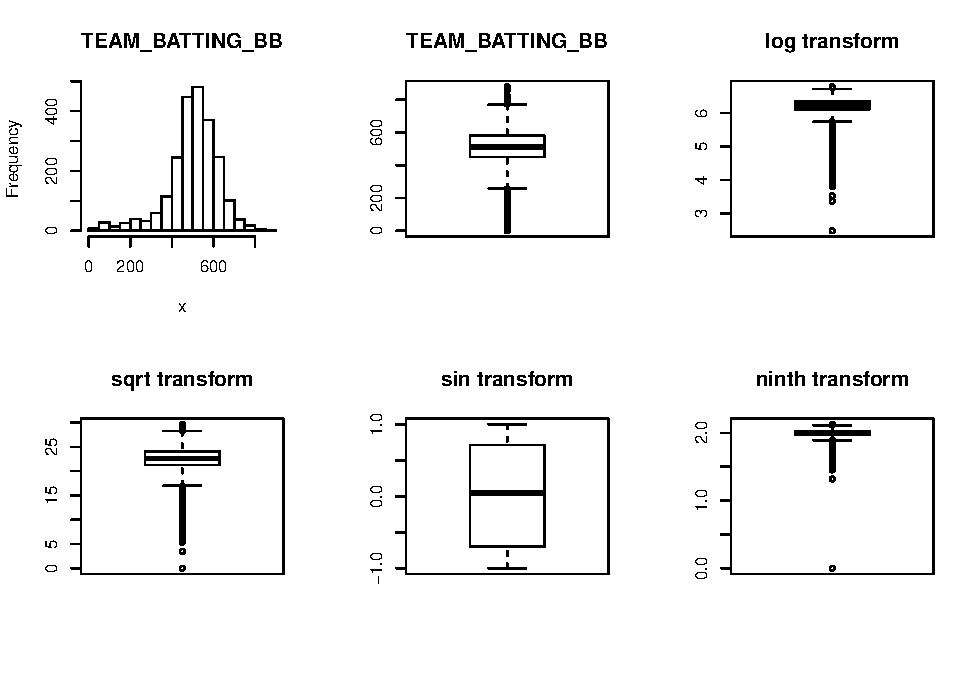
\includegraphics{apa3_files/figure-latex/unnamed-chunk-9-1.pdf}\\

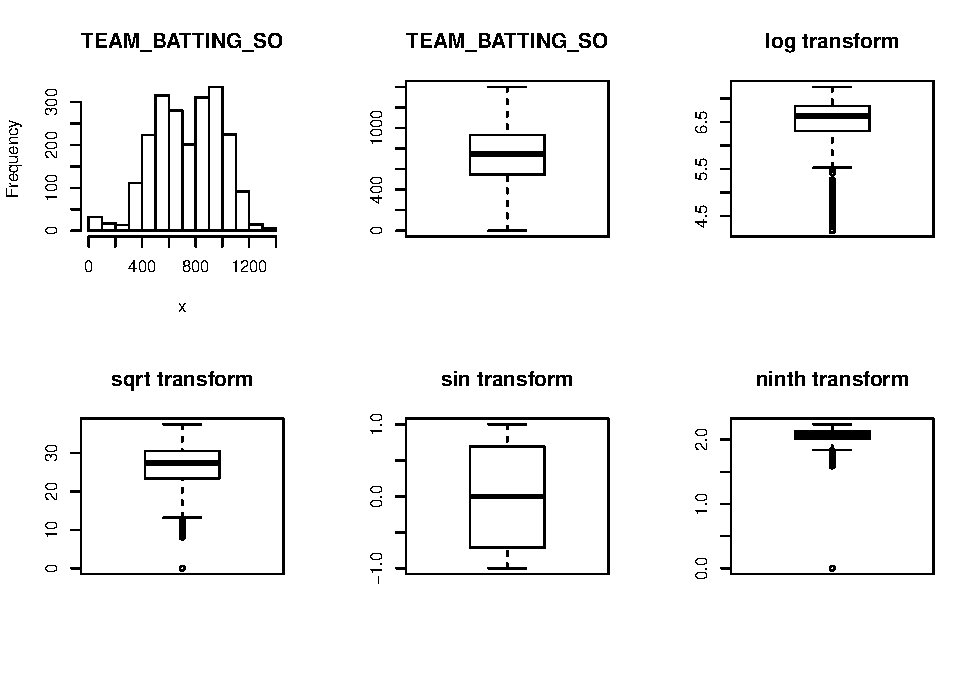
\includegraphics{apa3_files/figure-latex/unnamed-chunk-10-1.pdf}!\href{apa3_files/figure-latex/unnamed-chunk-10-2.pdf}{}!\href{apa3_files/figure-latex/unnamed-chunk-10-3.pdf}{}!\href{apa3_files/figure-latex/unnamed-chunk-10-4.pdf}{}!\href{apa3_files/figure-latex/unnamed-chunk-10-5.pdf}{}!\href{apa3_files/figure-latex/unnamed-chunk-10-6.pdf}{}!\href{apa3_files/figure-latex/unnamed-chunk-10-7.pdf}{}!\href{apa3_files/figure-latex/unnamed-chunk-10-8.pdf}{}\\
 \#\#\#2.6 Analysis the link function\\
 In this section, we will investigate how our initial data aligns with a
typical logistic model plot.

Recall the Logistic Regression is part of a larger class of algorithms
known as Generalized Linear Model (glm). The fundamental equation of
generalized linear model is:

\(g(E(y)) = a+ Bx_1+B_2x_2+ B_3x_3+...\)

where, g() is the link function, E(y) is the expectation of target
variable and \(B_0 + B_1x_1 + B_2x_2+B_3x_3\) is the linear predictor (
\(B_0,B_1,B_2, B_3\) to be predicted). The role of link function is to
\enquote{link} the expectation of y to linear predictor.

In logistic regression, we are only concerned about the probability of
outcome dependent variable ( success or failure). As described above,
g() is the link function. This function is established using two things:
Probability of Success (p) and Probability of Failure (1-p). p should
meet following criteria: It must always be positive (since p
\textgreater{}= 0) It must always be less than equals to 1 (since p
\textless{}= 1).

Now let's investigate how our initial data model aligns with the above
criteria. In other words, we will plot regression model plots for each
variable and compare it to a typical logistic model plot:

The main objective in the transformations is to achieve linear
relationships with the dependent variable (or, really, with its logit).

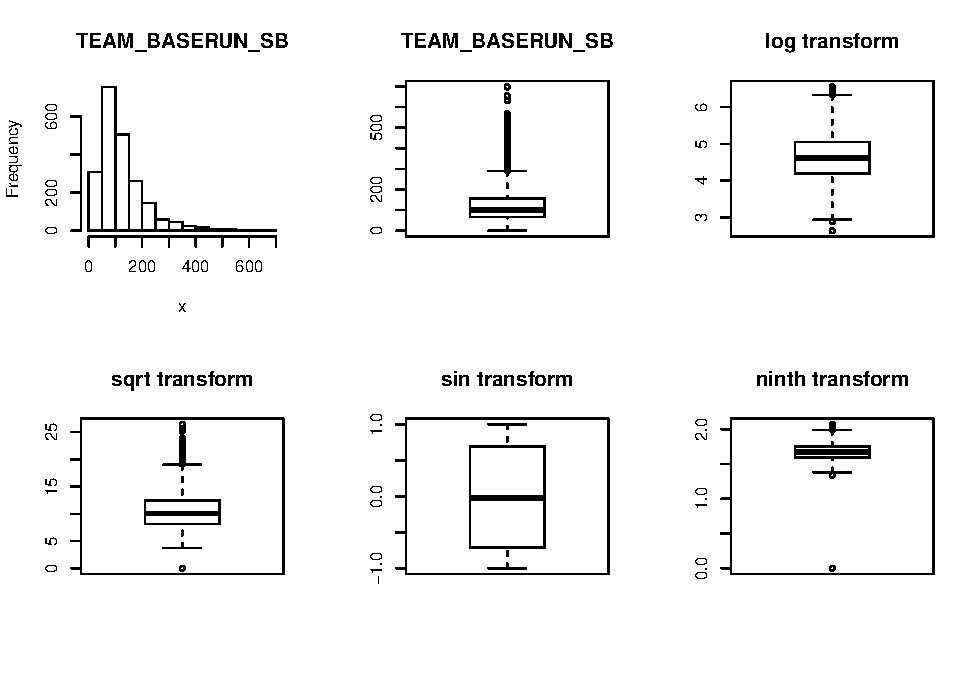
\includegraphics{apa3_files/figure-latex/unnamed-chunk-11-1.pdf}!\href{apa3_files/figure-latex/unnamed-chunk-11-2.pdf}{}!\href{apa3_files/figure-latex/unnamed-chunk-11-3.pdf}{}!\href{apa3_files/figure-latex/unnamed-chunk-11-4.pdf}{}!\href{apa3_files/figure-latex/unnamed-chunk-11-5.pdf}{}!\href{apa3_files/figure-latex/unnamed-chunk-11-6.pdf}{}!\href{apa3_files/figure-latex/unnamed-chunk-11-7.pdf}{}!\href{apa3_files/figure-latex/unnamed-chunk-11-8.pdf}{}\\
 \#\#3 Build Models

In this section, we will create 3 models. Aside from using original and
transformed data, we will also be using different methods and functions
such as Linear Discriminant Analysis, step function, and logit function
to enhance our models.

Below is our model definition:

-Model 1- This model will be created using all the variables in train
data set with logit function GLM.

-Model 2: This model step function will be used to enhance the model 1.

-Model 3- This model will be created using calssification and regression
tree.

\subsubsection{3.1 Model 1}\label{model-1}

Taking the treated data and splitting into 80/20 to train model and
validate the data.

Call: glm(formula = y \textasciitilde{} ., family = binomial(link =
\enquote{logit}), data = DS\_TARGET\_FLAG\_TRAIN)

Deviance Residuals: Min 1Q Median 3Q Max\\
-5.9813 -0.2993 -0.1864 -0.1341 3.3267

Coefficients: (11 not defined because of singularities) Estimate Std.
Error z value Pr(\textgreater{}\textbar{}z\textbar{})\\
(Intercept) -2.206e+02 1.225e+02 -1.800 0.071872 .\\
age 1.059e-03 2.712e-03 0.390 0.696177\\
duration 4.655e-03 8.280e-05 56.220 \textless{} 2e-16 \textbf{\emph{
campaign -4.301e-02 1.303e-02 -3.302 0.000960 }} pdays -1.973e-02
2.026e-02 -0.973 0.330334\\
previous -6.319e-02 6.878e-02 -0.919 0.358304\\
emp.var.rate -1.698e+00 1.588e-01 -10.696 \textless{} 2e-16
\textbf{\emph{ cons.price.idx 2.157e+00 2.828e-01 7.626 2.43e-14 }}
cons.conf.idx 2.196e-02 8.701e-03 2.524 0.011617 *\\
euribor3m 2.814e-01 1.460e-01 1.928 0.053818 .\\
nr.employed 5.399e-03 3.498e-03 1.543 0.122727\\
job\_housemaid -4.131e-01 2.019e-01 -2.046 0.040753 *\\
job\_services -3.466e-01 1.401e-01 -2.475 0.013328 *\\
job\_admin. -2.500e-01 1.232e-01 -2.029 0.042506 *\\
\texttt{job\_blue-collar} -4.859e-01 1.320e-01 -3.681 0.000233
\textbf{\emph{ job\_technician -2.597e-01 1.312e-01 -1.980 0.047684 }\\
job\_retired -3.081e-02 1.699e-01 -0.181 0.856065\\
job\_management -2.566e-01 1.483e-01 -1.730 0.083551 .\\
job\_unemployed -2.599e-01 1.782e-01 -1.459 0.144675\\
\texttt{job\_self-employed} -3.849e-01 1.712e-01 -2.248 0.024571 *\\
job\_unknown -4.242e-01 2.848e-01 -1.490 0.136340\\
job\_entrepreneur -3.961e-01 1.796e-01 -2.205 0.027442 *\\
job\_student NA NA NA NA\\
marital\_married 2.842e-01 4.873e-01 0.583 0.559762\\
marital\_single 3.658e-01 4.883e-01 0.749 0.453869\\
marital\_divorced 2.980e-01 4.917e-01 0.606 0.544487\\
marital\_unknown NA NA NA NA\\
education\_illiterate 2.121e-01 9.912e-01 0.214 0.830518\\
education\_unknown 1.068e-03 1.119e-01 0.010 0.992385\\
education\_primary -1.487e-01 8.573e-02 -1.734 0.082875 .\\
education\_secondary -1.528e-01 5.824e-02 -2.624 0.008689 }
education\_tertiary NA NA NA NA\\
default\_no 7.336e+00 1.131e+02 0.065 0.948283\\
default\_unknown 6.966e+00 1.131e+02 0.062 0.950892\\
default\_yes NA NA NA NA\\
housing\_no -2.184e-02 1.607e-01 -0.136 0.891904\\
housing\_yes -1.775e-02 1.595e-01 -0.111 0.911397\\
housing\_unknown NA NA NA NA\\
loan\_no 6.178e-02 6.417e-02 0.963 0.335699\\
loan\_yes NA NA NA NA\\
loan\_unknown NA NA NA NA\\
contact\_telephone -6.139e-01 8.529e-02 -7.198 6.11e-13 \textbf{\emph{
contact\_cellular NA NA NA NA\\
month\_may -7.295e-01 1.695e-01 -4.303 1.69e-05 }} month\_jun -8.126e-01
2.638e-01 -3.081 0.002065 ** month\_jul -1.307e-01 1.947e-01 -0.671
0.502243\\
month\_aug 5.923e-01 1.572e-01 3.767 0.000165 \textbf{\emph{ month\_oct
-6.020e-02 1.573e-01 -0.383 0.701942\\
month\_nov -6.410e-01 1.683e-01 -3.809 0.000139 }} month\_dec 1.460e-01
2.337e-01 0.624 0.532322\\
month\_mar 1.745e+00 1.717e-01 10.164 \textless{} 2e-16 \textbf{\emph{
month\_apr -3.229e-01 2.002e-01 -1.613 0.106732\\
month\_sep NA NA NA NA\\
day\_of\_week\_mon -1.688e-01 7.382e-02 -2.287 0.022223 }\\
day\_of\_week\_tue 5.239e-02 7.358e-02 0.712 0.476411\\
day\_of\_week\_wed 1.706e-01 7.302e-02 2.336 0.019496 *\\
day\_of\_week\_thu 2.541e-02 7.123e-02 0.357 0.721301\\
day\_of\_week\_fri NA NA NA NA\\
previous\_contact -1.845e+01 2.003e+01 -0.921 0.357110\\
poutcome\_nonexistent -3.273e-01 2.552e-01 -1.283 0.199611\\
poutcome\_failure -8.008e-01 2.573e-01 -3.113 0.001853 }
poutcome\_success NA NA NA NA\\
--- Signif. codes: 0 \enquote{\emph{\textbf{' 0.001 '}' 0.01 '}} 0.05
\enquote{.} 0.1 \enquote{} 1

(Dispersion parameter for binomial family taken to be 1)

\begin{verbatim}
Null deviance: 23294  on 32949  degrees of freedom
\end{verbatim}

Residual deviance: 13674 on 32899 degrees of freedom AIC: 13776

Number of Fisher Scoring iterations: 10

Analysis of Deviance Table

Model: binomial, link: logit

Response: y

Terms added sequentially (first to last)

\begin{verbatim}
                 Df Deviance Resid. Df Resid. Dev  Pr(>Chi)    
\end{verbatim}

NULL 32949 23294\\
age 1 26.1 32948 23268 3.159e-07 \textbf{\emph{ duration 1 3927.1 32947
19340 \textless{} 2.2e-16 }} campaign 1 182.3 32946 19158 \textless{}
2.2e-16 \textbf{\emph{ pdays 1 2044.5 32945 17114 \textless{} 2.2e-16 }}
previous 1 78.9 32944 17035 \textless{} 2.2e-16 \textbf{\emph{
emp.var.rate 1 1946.6 32943 15088 \textless{} 2.2e-16 }} cons.price.idx
1 399.3 32942 14689 \textless{} 2.2e-16 \textbf{\emph{ cons.conf.idx 1
125.3 32941 14564 \textless{} 2.2e-16 }} euribor3m 1 22.2 32940 14541
2.453e-06 \textbf{\emph{ nr.employed 1 21.7 32939 14520 3.162e-06 }}
job\_housemaid 1 1.9 32938 14518 0.1628500\\
job\_services 1 7.6 32937 14510 0.0057626 ** job\_admin. 1 8.7 32936
14501 0.0032324 ** \texttt{job\_blue-collar} 1 78.7 32935 14423
\textless{} 2.2e-16 \textbf{\emph{ job\_technician 1 0.1 32934 14423
0.8164324\\
job\_retired 1 12.4 32933 14410 0.0004189 }} job\_management 1 0.0 32932
14410 0.9031846\\
job\_unemployed 1 0.0 32931 14410 0.8323131\\
\texttt{job\_self-employed} 1 0.7 32930 14409 0.3879983\\
job\_unknown 1 0.7 32929 14409 0.4061109\\
job\_entrepreneur 1 12.3 32928 14396 0.0004446 \textbf{\emph{
job\_student 0 0.0 32928 14396\\
marital\_married 1 6.3 32927 14390 0.0121511 }\\
marital\_single 1 3.1 32926 14387 0.0765905 .\\
marital\_divorced 1 0.1 32925 14387 0.7014113\\
marital\_unknown 0 0.0 32925 14387\\
education\_illiterate 1 0.2 32924 14387 0.6947715\\
education\_unknown 1 1.6 32923 14385 0.2001283\\
education\_primary 1 2.2 32922 14383 0.1385503\\
education\_secondary 1 21.1 32921 14362 4.336e-06 }\emph{
education\_tertiary 0 0.0 32921 14362\\
default\_no 1 42.9 32920 14319 5.675e-11 }\textbf{ default\_unknown 1
0.0 32919 14319 0.8305794\\
default\_yes 1 0.0 32918 14319 1.0000000\\
housing\_no 0 0.0 32918 14319\\
housing\_yes 2 0.1 32916 14318 0.9470350\\
housing\_unknown 0 0.0 32916 14318\\
loan\_no 1 1.3 32915 14317 0.2472729\\
loan\_yes 0 0.0 32915 14317\\
loan\_unknown 0 0.0 32915 14317\\
contact\_telephone 1 149.5 32914 14168 \textless{} 2.2e-16 }\emph{
contact\_cellular 0 0.0 32914 14168\\
month\_may 1 177.0 32913 13991 \textless{} 2.2e-16 }\textbf{ month\_jun
1 0.0 32912 13991 0.8444638\\
month\_jul 1 2.9 32911 13988 0.0896473 .\\
month\_aug 1 21.1 32910 13967 4.345e-06 }\emph{ month\_oct 1 0.0 32909
13967 1.0000000\\
month\_nov 1 36.5 32908 13930 1.495e-09 }\textbf{ month\_dec 1 0.1 32907
13930 0.7209786\\
month\_mar 1 198.9 32906 13731 \textless{} 2.2e-16 }\emph{ month\_apr 1
3.1 32905 13728 0.0769399 .\\
month\_sep 0 0.0 32905 13728\\
day\_of\_week\_mon 1 16.6 32904 13711 4.672e-05 }\textbf{
day\_of\_week\_tue 1 0.1 32903 13711 0.7999177\\
day\_of\_week\_wed 1 6.6 32902 13705 0.0101931 *\\
day\_of\_week\_thu 0 0.3 32902 13704\\
day\_of\_week\_fri 0 0.0 32902 13704\\
previous\_contact 2 5.8 32900 13699 0.0564142 .\\
poutcome\_nonexistent 1 14.7 32899 13684 0.0001267 }* poutcome\_failure
0 9.7 32899 13674\\
poutcome\_success 0 0.0 32899 13674\\
--- Signif. codes: 0 \enquote{\emph{\textbf{' 0.001 '}' 0.01 '}} 0.05
\enquote{.} 0.1 \enquote{} 1 llh llhNull G2 McFadden r2ML -6.837189e+03
-1.164683e+04 9.619284e+03 4.129571e-01 2.531835e-01 r2CU 4.995246e-01
{[}1{]} \enquote{Accuracy 0.910779315367808}

\paragraph{3.2 Model 2}\label{model-2}

\subsubsection{3.3 Model 3}\label{model-3}

\subsection{4 Evaluate Models}\label{evaluate-models}

\subsection*{5 Select Models}\label{select-models}
\addcontentsline{toc}{subsection}{5 Select Models}

\hypertarget{refs}{}
\hypertarget{ref-R-papaja}{}
Aust, F., \& Barth, M. (2015). \emph{Papaja: Create aPA manuscripts with
rMarkdown}. Retrieved from \url{https://github.com/crsh/papaja}

\hypertarget{ref-R-base}{}
R Core Team. (2016). \emph{R: A language and environment for statistical
computing}. Vienna, Austria: R Foundation for Statistical Computing.
Retrieved from \url{https://www.R-project.org/}



\end{document}
